\documentclass[class=book, crop=false]{standalone}
\usepackage[subpreambles=true]{standalone}
\usepackage[utf8]{inputenc}
\usepackage{import}
\usepackage[ruled,vlined]{algorithm2e}

\usepackage{amsmath}
\usepackage{amssymb}
\usepackage[margin=1.2in]{geometry}
\usepackage[sorting = none,
            doi = true  %lesedato for url-adresse
            ]{biblatex} %none gir bibliografi i sitert rekkefølge
\addbibresource{reference.bib}
\usepackage{csquotes}
\usepackage{pgfplots}
\usepackage{pgfplotstable}

\pgfplotsset{compat=1.15}

\begin{document}
\section{Performance of the trained agent}
The results from section \ref{section:result:config1} show that the trained agent is able to reduce the number of safety violation by 10\%. However, the trained agent is only able to reduce violations of voltage safety margins, not current violations. In fact, it increases the number of current violations by 18 \%. Still, there are large differences in terms of the quantity and magnitude of the current and voltage safety violations. There are almost 7 times more voltage violations than current violations. This is of course dependent on the voltage bounds that are used for defining the voltage cost. In this case the voltage bounds are chosen to be 0.95 and 1.05 pu. Although there are many more voltage violations in a normal day, the average current violation is more severe. Specifically, the mean current cost is almost 5 times greater than the mean voltage cost. The nature of the transmission in terms of violations is therefore: the current violation are sparse and severe, while the voltage violations are numerous and faint. 

Why is the trained agent better at avoiding voltage violation than current violations? A possible reason is that the agent is penalised more for voltage violations on average. The total voltage costs is 40 \% greater than the total current cost, because they are more frequent. It is logical that the agent learns a behaviour that reduces the most punishing term, namely the voltage cost. As stated in section \ref{section:config1:current_violations}, the trained agent only learned the appropriate behaviour in periods of peak demand, i.e reducing the demand so that less power need to be imported from the grid.

The agent was worsening the situation in periods of peak solar production. The desired behaviour in such a situation is to increase the demand, so that less excess solar power needs to be exported to the grid. Consequently, the trained agent decreases the demand in periods of peak solar production, since the number of line overload increases. It is possible that the learned behaviour simply is to decrease the demand at all times. It is possible, especially considering that the energy imbalance in the system is negative, as shown in figure \ref{fig:results:configuration1_energy_imbalance}. Figure \ref{fig:discussion:config1_action_hour} shows the mean action taken by the agent throughout a the day in the 500 episode simulation. The pattern of the actions are good, because the it goes down up during peak solar producing (hour 12) and down during peak demand in the afternoon. However, the change in demand during peak demand is still negative. The action signal seem to have a negative bias. It is also worth noting that the mean action is quite low in absolute magnitude. In other words, the agent is not using the entire available flexibility in the system, at least not on a global scale.

\begin{figure}[h]
    \center
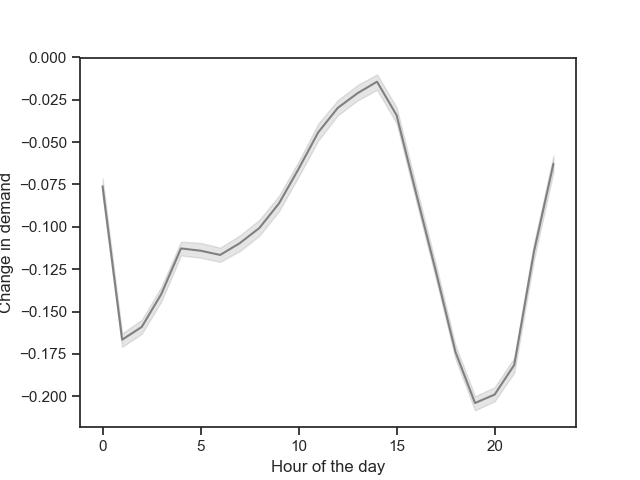
\includegraphics[height=8cm, width=12cm]{figures/config1_action_hour.png}
    \caption[size = 9]{Hourly mean values for the change in demand at the buses in the net, as determined by the trained reinforcement agent}
    \label{fig:discussion:config1_action_hour}
\end{figure}


\section{Nominal values for consumption and production}
The action of the reinforcement agent determines the percentage change in demand at each load in the interval $[-f,f]$, where $f$ is the flexibility of demand. Naturally, the load is varying a lot throughout a day, but the nominal demand also vary a lot from bus to bus. Figure \ref{fig:discussion:nominal_load} shows the values for nominal apparent power at each bus bar in the power system, as predefined in \texttt{pandapower}.

\begin{figure}[h]
    \center
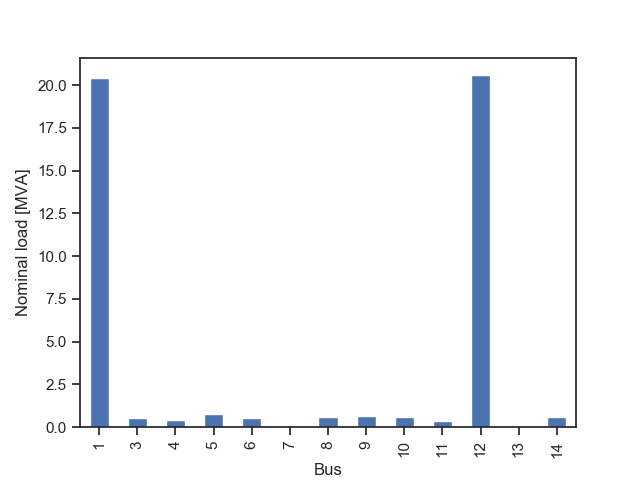
\includegraphics[height=8cm, width=12cm]{figures/nominal_load.png}
    \caption[size = 9]{Bar plot of the nominal apparent power at each bus in the CIGRE network}
    \label{fig:discussion:nominal_load}
\end{figure}

Bus 1 and 12 clearly stand out, and account for nearly 90 \% of the total system demand. For simplicity, they will be referred to as the dominant buses due their large demand. Note that there is no solar power connected to them. Because each action variable is scaled up by the nominal load, it is clear that action +1 for the dominant buses has a much larger impact in terms of absolute power change than it has on the rest of the buses. As shown in figure \ref{fig:discussion:cigre_network_dominant}, The dominant buses are placed in the top of each feeder 1 and feeder 2, connected to each their 220/22 kV transformer. 

\begin{figure}[ht]
    \center
    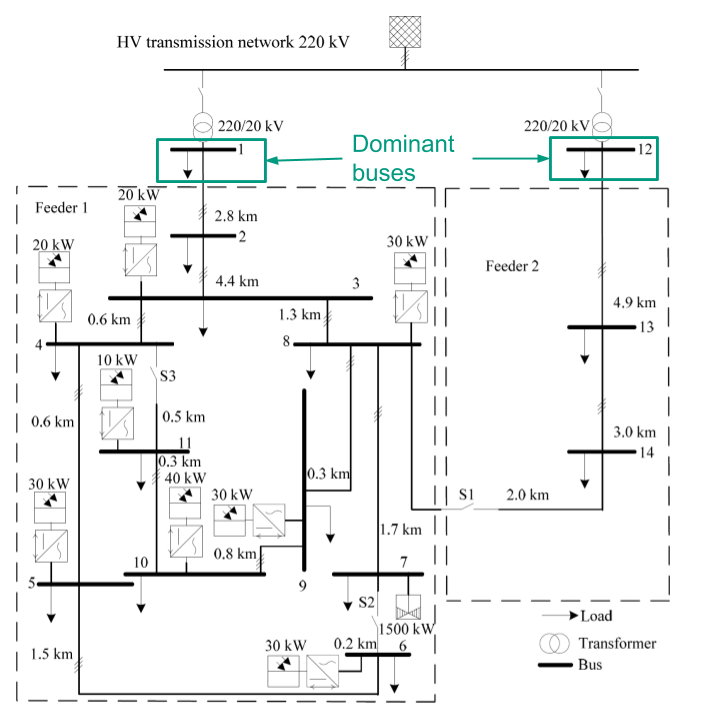
\includegraphics[height=14cm, width=13.5cm]{figures/cigre_network_dominant.png}
    \caption[size = 9]{CIGRE network with solar and wind power that is used in the reinforcement learning algorithm \cite{cigre}}
    \label{fig:discussion:cigre_network_dominant}
\end{figure}
It might seem troubling that these buses have a much larger nominal values. However, because they are placed next to the grid, they do not affect the line current in the rest of the system much. For instance, if the load at bus 1 is doubled, the current through the transformer approximately doubles to supply the demand. Naturally, this could be very critical for the transformer, but it has a small effect on the line currents in the power system, because the rest of the loads still draw the same amount of power from the grid,. The current effect of changing the demand at bus 1 and 12 are not that decisive as one first might think, due to their position close to the external grid. On the other hand, they can greatly affect the voltage magnitudes in the grid. Figure \ref{fig:discussion:double_large_load} illustrates the effect increasing the demand at the dominant buses has on the rest of the buses. The predefined demand values are used for solving the power flow equations in situation A, while they are doubled for the dominant buses (1 and 12) in situation B.

\begin{figure}[h]
    \center
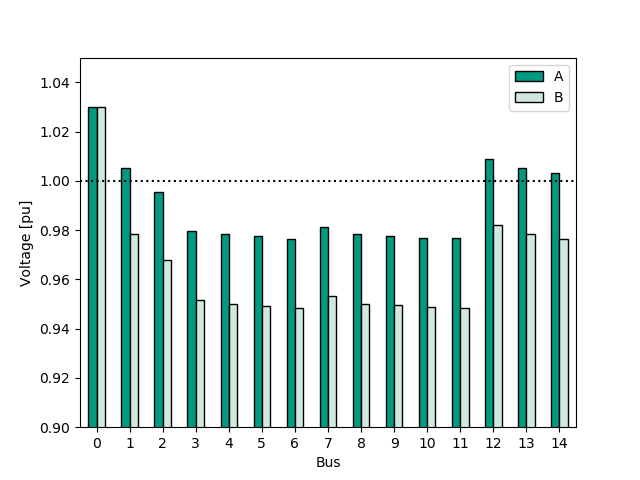
\includegraphics[height=8cm, width=12cm]{figures/double_large_load.png}
    \caption[size = 9]{Bar plot for each of the buses showing their voltage magnitude in nominal operation (A) and after the demand at bus 1 and 12 in \ref{fig:discussion:cigre_network_dominant} is doubled (B). Note that the second axis is truncated}
    \label{fig:discussion:double_large_load}
\end{figure}
The dominant buses serve as the starting point for the voltage magnitudes because they are at the beginning of the two feeders. This is true because there are only PQ-buses in the system and no voltage regulating units. The voltage is static at the external grid, and gradually falls as we move down the feeders. When bus 1 doubles its demand, it reduces its voltage magnitude which in turn propagates down the feeder and affects all buses in the feeder. The difference in voltage magnitude at each bus before and after the demand increase is almost linear. The reinforcement agent is not able to double the demand, but figure \ref{fig:discussion:double_large_load} illustrates the decisive effect of the dominant buses in terms of voltage magnitudes. Let the voltage and current impact of a bus respectively be defined as the sum of the changes in voltage and current load in the net when modifying the demand at that bus by a certain percent. Note that the rest of the buses are left unchanged when calculating the impact. The predefined demand values in the CIGRE network correspond to an hour of peak demand, with low voltage magnitudes in the grid. Increasing the demand at a bus with a high voltage impact has a large potential of pulling the voltage magnitudes into the safety bounds. The same is true for a bus with a high current impact. Figure \ref{fig:discussion:voltage_impact} plots the voltage impact for each bus where the flexibility of demand ranges from -20 to +20 \%. The lower part of the box plots correspond to increasing the demand by 20 \%, since increasing the demand in peak demand lowers the voltage magnitudes in the grid. As already discussed, bus 1 have a very large voltage impact, because it is at the top of feeder 1. 

\begin{figure}[h]
    \center
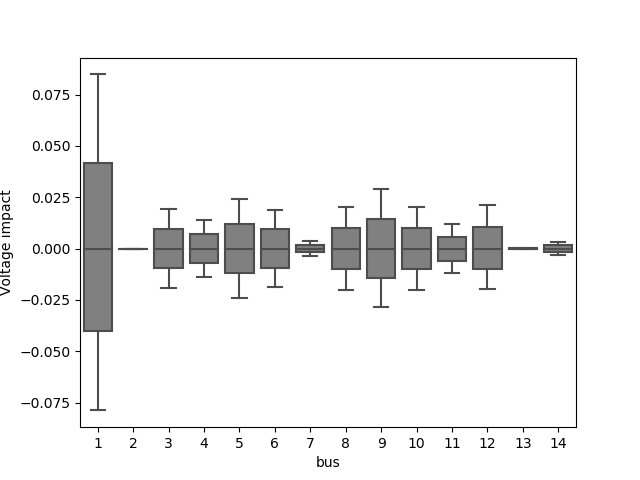
\includegraphics[height=8cm, width=12cm]{figures/voltage_impact.png}
    \caption[size = 9]{Box plot for each bus bar showing the voltage importance for a flexibility of demand ranging from -20 to + 20 \%}
    \label{fig:discussion:voltage_impact}
\end{figure}

Figure \ref{fig:discussion:current_impact} plots the current impact for the buses in the system. The buses with highest current impact (5,6,9,10) are all located far down in feeder 1. A change in demand at them has consequences for several lines, because the current they draw must travel through the lines in the top of the feeder. Has the trained agent learned the current and voltage impact of the buses?    


\begin{figure}[h]
    \center
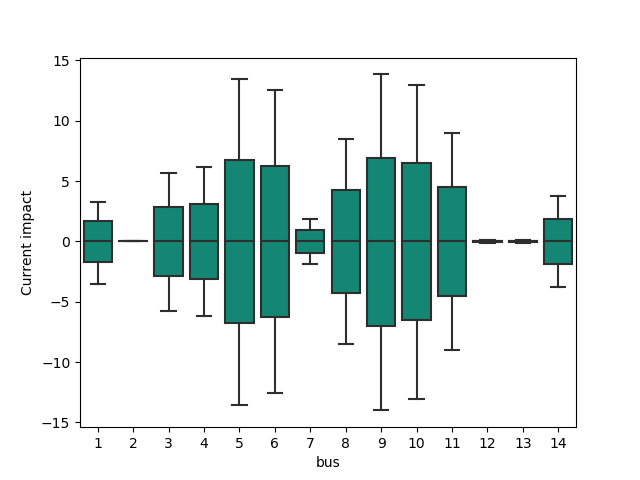
\includegraphics[height=8cm, width=12cm]{figures/current_impact.png}
    \caption[size = 9]{Box plot for each bus bar showing the current importance for a demand change ranging from -20 to + 20 \%}
    \label{fig:discussion:current_impact}
\end{figure}

\section{Solar power production}
The nominal solar production level predefined in the network is scaled up by a factor of 40. This is done to challenge the grid by increasing the number of current and voltage violations in hours of peak solar production. The nominal values for solar production and consumption at the solar producing buses are presented in figure \ref{fig:discussion:nominal_sgen}


\begin{figure}[h]
    \center
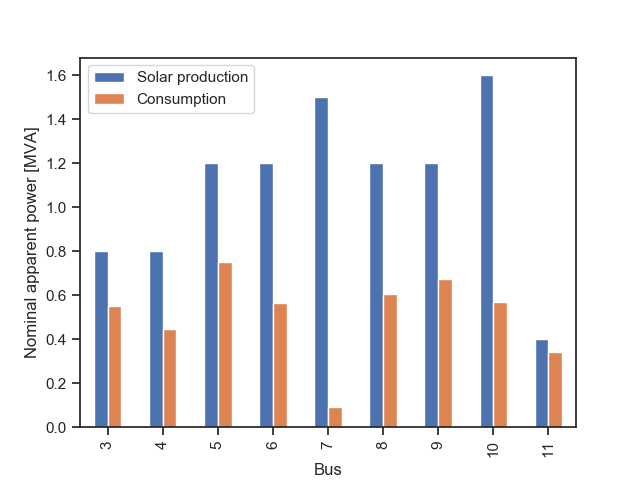
\includegraphics[height=8cm, width=12cm]{figures/nominal_sgen.png}
    \caption[size = 9]{Bar plot of the nominal apparent power consumption and solar production at solar producing buses in the grid}
    \label{fig:discussion:nominal_sgen}
\end{figure}




\section{State representation}
There are many different ways of constructing the state space in the reinforcement agent. In section \ref{section:problem:state_space} several candidates for the state space were introduced, such as the the bus space. The bus space consists of the active power $P$, reactive power $Q$, voltage magnitude $|U|$ and phase angle $\delta$ for all the buses in the system. It was not included in the state space of the trained reinforcement agent. A reason for this is that the current bus state tells nothing relevant about the future. Naturally, there is a correlation between the bus state and the subsequent state. For instance, during peak demand in the afternoon, the demand between two hours are highly correlated, which in turns determines the bus states. However, this information can be found in the demand forecasts. In some sense, the bus state in the current time step is redundant. During peak solar production, we can have an hour with heavy production from solar units, but in the next hour the forecasts says that there will be cloudy. It is not possible to predict the clouds from the bus state. The predictive information is hidden in the forecast. Of course, the forecasts can be used to calculate the predicted bus state, which can be helpful information for the agent. However, this will slow down the training process, because the power flows equation must be solved, possibly several times if many future bus states are going to be predicted. 
- Why several hour forecast?
- Include flexibility, price of flexibility, bus-wise features. 


\section{Reward function}
The reward function is designed to penalise violations of safety margins in the grid. Specifically, current overloads and violations of voltage safety margin are the factors that are used to calculate the reward signal. There are however two transformers in the grid, that also should be included in the reward functions. Transformer are not fireproof. \texttt{pandapower} has a result table for the transformer, that easily could be integrated in the reward function.

\end{document}